% https://logic.pdmi.ras.ru/~sergey/teaching/mdcsclub/06-combinatorial.pdf

Современные исследования . Приведем краткое описание постановок разбирающие.

\subsubsection{Кобминаторные аукционы}

\begin{figure}[h]
    \centering
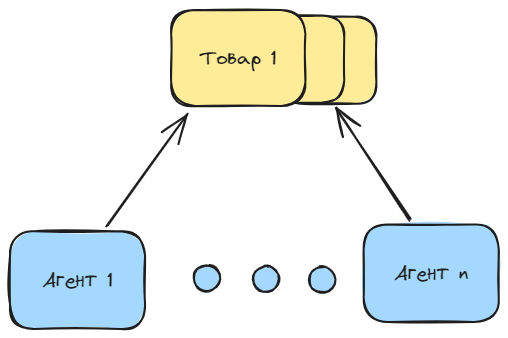
\includegraphics[width=0.5\textwidth]{assets/auctions/combinatorial.excalidraw.png}
    \caption{Комбинаторные аукционы подразумевает различие в полезности агента в обладание нескольких товаров}
    \label{сombinatorial}
\end{figure}

\textit{Комбинаторные аукционы} \ref{сombinatorial} обобщают постановку классического аукциона

    
\textit{Дополняющие вещи} определяют

\textit{Взаимозаменяемые вещи}


\subsubsection{Обратные аукционы}


\begin{figure}[h]
    \centering
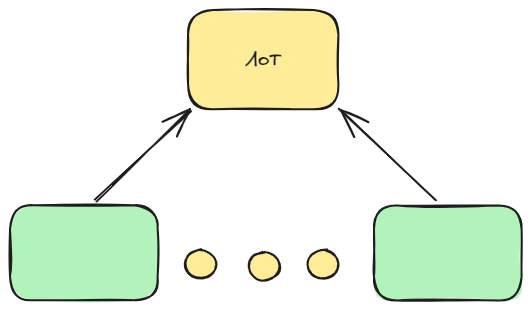
\includegraphics[width=0.5\textwidth]{assets/auctions/reversed.excalidraw.png}
    \caption{Обратные аукционы}
    \label{reversed}
\end{figure}

В обратном аукционе поставщики соревнуются за право на выполнение лота



